\documentclass[11pt]{article}
\usepackage[utf8]{inputenc}
\usepackage[top = 2cm,left=3cm,right=3cm,bottom=2cm,]{geometry}
\usepackage{amsfonts,amsmath,amssymb,xfrac,subcaption,graphicx,placeins,xcolor}
\usepackage{hyperref}

\title{Homework 2 \\ \small{Applied Macroeconomics: Micro Data for Macro Models}\thanks{The full replication files for this paper can be found in https://github.com/jmquintero925/Applied-Macro.}}
\author{Jose M. Quintero\thanks{\textcolor{blue}{Big thanks to Issac Norwich for hearing all my complains about this Problem Set. Stata sucks and cannot handle dates. Long live MATLAB.} }}
\date{}


\begin{document}
\vspace{-1cm}\maketitle\vspace{-1cm}

\section{House price growth}
In their paper, ``Regional Heterogeneity and the Refinancing Channel of Monetary Policy”, Beraja, Fuster, Hurst and Vavra show that the regional variation of home equity is a key determinant of refinancing mortgages. Specifically, they used the Great Financial crisis shock to show that the areas with more home equity where more likely to experiences higher waves of refinancing. The underlying mechanism is that homeowners use cash-out refinance mortgages to make their  liquidate their assets and smooth consumption. 
\begin{figure}[htb]
    \centering
    \caption{Price Growth and Mortgages Refinanced}
    \label{hw2:fig1}
    \begin{subfigure}[b]{0.45\textwidth}
            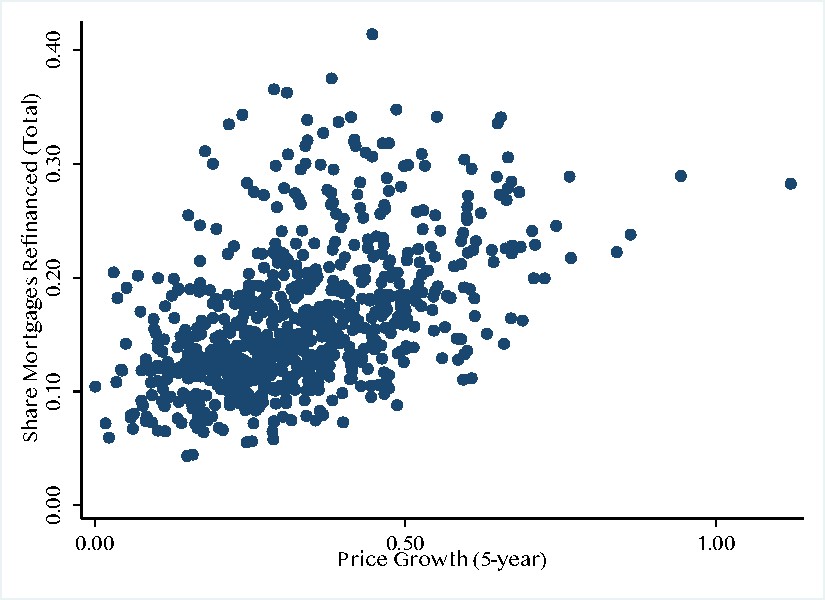
\includegraphics[width=\textwidth]{Figures/price_growth.pdf}
            \caption{Mortgages Refinanced}
        \end{subfigure}
        \begin{subfigure}[b]{0.45\textwidth}
            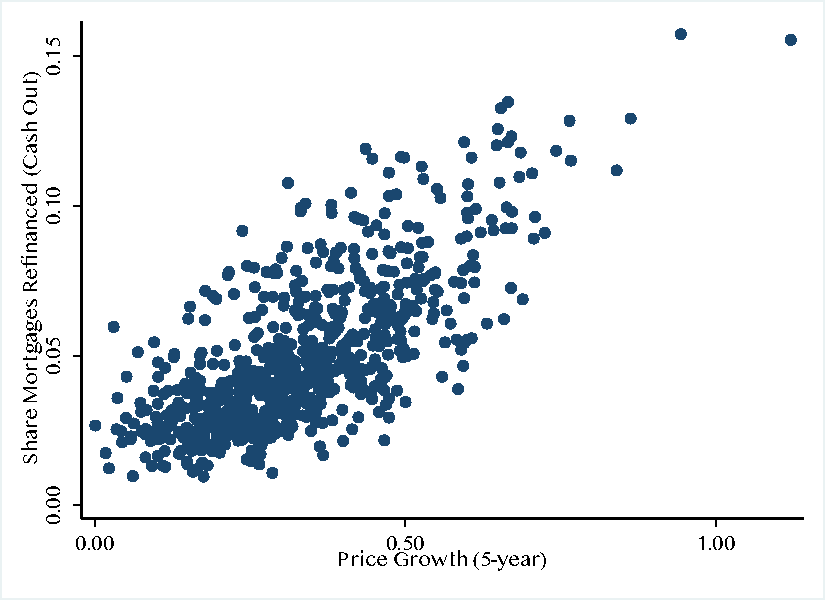
\includegraphics[width=\textwidth]{Figures/price_growth2.pdf}
            \caption{Cash Out Mortgages Refinanced}
        \end{subfigure}
\end{figure}
\FloatBarrier
We try to unveil this same fact using the COVID crisis. The results are presented in Figure \ref{hw2:fig1} and Table \ref{hw2:}. Both of the findings are consistent with the results in the original paper. 
\begin{table}[htb]
    \centering
    \caption{Price Growth and Mortgages Refinanced}
    \label{hw2:}
    \small{
    \begin{tabular}{l*{2}{c}}
\hline\hline
&\multicolumn{1}{c}{(1)}&\multicolumn{1}{c}{(2)}\\
& Share Mortgages Refinanced   & Share Mortgages Refinanced \\
& (Total) & (Cash Out) \\ 
\hline
Price Growth  &       0.192\sym{***}	&       0.126\sym{***}\\
            			&    (0.0282)         		&   (0.00959)         \\
Constant      	&       0.120\sym{***}	&      0.0108\sym{***}\\
            			&    (0.0122)         		&   (0.00321)         \\
\hline
\(N\)       		&   748         				&    748         \\
\hline\hline
\multicolumn{3}{l}{\footnotesize Standard errors in parentheses and clustered at the regional level.}\\
\multicolumn{3}{l}{\footnotesize \sym{*} \(p<0.05\), \sym{**} \(p<0.01\), \sym{***} \(p<0.001\)}\\
\end{tabular}


    }
\end{table}
\FloatBarrier
Note that the independent variable is price growth, as argued in the original paper, it captures the growth of home equity. The regressions in Table \ref{hw2:} are consistent with the ones in the original paper as the places that experience a higher household equity growth are most likely to refinance. 
\section{Housing equity}
Now in this section we focus on the relation between price growth and leverage. Recall that price growth is proxying for equity growth. For instance, the original paper finds a strong correlation between equity and leverage. 
\begin{figure}[htb]
    \centering
    \caption{Leverage and Price Growth}
    \label{hw2:fig2}
    \begin{subfigure}[b]{0.47\textwidth}
            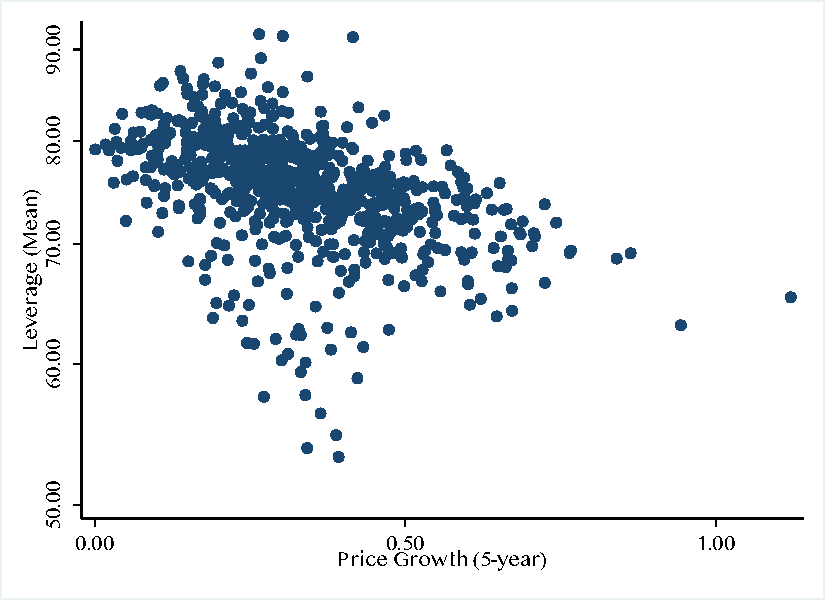
\includegraphics[width=\textwidth]{Figures/leverage_mean.pdf}
            \caption{Mean}
        \end{subfigure}
        \begin{subfigure}[b]{0.47\textwidth}
            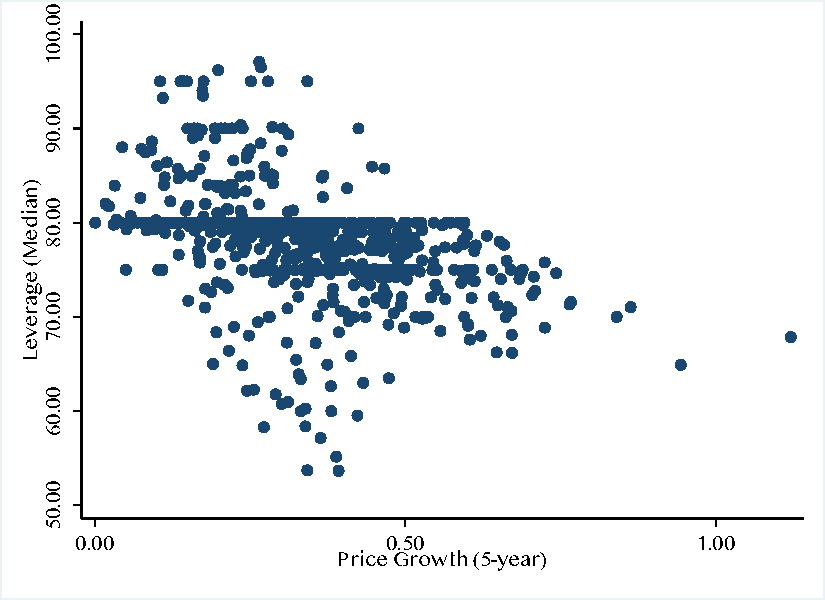
\includegraphics[width=\textwidth]{Figures/leverage_median.pdf}
            \caption{Median}
        \end{subfigure}
\end{figure}
\FloatBarrier
We use loan to value ratio as a measure of leverage similar to the original paper. Note that our results in Table \ref{hw2:tab2} and Figure \ref{hw2:fig2} are consistent to the findings in the original paper as leverage is negatively correlated with price growth. This correlation is statistically significant, suggesting that using price growth to understand the propensity to refinance already accounts for differences in leverage. 
\begin{table}[htb]
    \centering
    \caption{Leverage and Mortgages Refinanced}
    \label{hw2:tab2}
    \small{
    {
\def\sym#1{\ifmmode^{#1}\else\(^{#1}\)\fi}
\begin{tabular}{l*{2}{c}}
\hline\hline
& Share Mortgages Refinanced   & Share Mortgages Refinanced \\
& (Total) & (Cash Out) \\ 
\hline
$\sfrac{\text{Loan}}{\text{Value}}$&    -0.00721\sym{***}&    -0.00262\sym{***}\\
            &  (0.000690)         &  (0.000306)         \\
Constant     &       0.731\sym{***}&       0.252\sym{***}\\
            &    (0.0571)         &    (0.0248)         \\
\hline
\(N\)       &         766         &         766         \\
\hline\hline
\multicolumn{3}{l}{\footnotesize Standard errors in parentheses and clustered at the regional level.}\\
\multicolumn{3}{l}{\footnotesize \sym{*} \(p<0.05\), \sym{**} \(p<0.01\), \sym{***} \(p<0.001\)}\\
\end{tabular}
}

    }
\end{table}

\section{Data and others}
One limitation of the HDMA data is that it does not allow to link loan to borrowers. If one borrower has multiple loans, it can create noise in the refinancing mechanism. Moreover, for this same reason, the magnitude of equity extracted is not observed and thus the proper response to the shock cannot be measure. Specifically, is hard to take a strong stance on whether consumers are actually using equity in their homes to smooth consumption or reorganizing the liquidity of their assets. Recall that during COVID, the price of several financial options drop drastically, (think stocks of companies) and forward looking agents could have opted to buy the low actions under the beliefs that the economy was going to bounce back. This particular scenario shows that refinancing could also be due to reallocation of liquidity in the agent portafolio. 


\end{document}


